\documentclass[12pt,a4paper]{article}
\usepackage[UTF8]{ctex}
\usepackage{listings}
\usepackage{xcolor}
\usepackage{graphicx}
\usepackage{appendix}

%代码段设置
\lstset{numbers=left,
basicstyle=\tiny,
numberstyle=\tiny,
keywordstyle=\color{blue!70},
commentstyle=\color{red!50!green!50!blue!50},
frame=single, rulesepcolor=\color{red!20!green!20!blue!20},
escapeinside=``
}

\graphicspath{ {images/} }
\usepackage{graphicx}
\usepackage{color,framed}%文本框
\usepackage{listings}
\usepackage{caption}
\usepackage{amssymb}
\usepackage{enumerate}
\usepackage{xcolor}
\usepackage{bm} 
\usepackage{lastpage}%获得总页数
\usepackage{fancyhdr}
\usepackage{tabularx}  
\usepackage{geometry}
\usepackage{minted}
\usepackage{graphics}
\usepackage{subfigure}
\usepackage{float}
\usepackage{pdfpages}
\usepackage{pgfplots}
\pgfplotsset{width=10cm,compat=1.9}
\usepackage{multirow}
\usepackage{footnote}
\usepackage{booktabs}

%-----------------------伪代码------------------
\usepackage{algorithm}  
\usepackage{algorithmicx}  
\usepackage{algpseudocode}  
\floatname{algorithm}{Algorithm}  
\renewcommand{\algorithmicrequire}{\textbf{Input:}}  
\renewcommand{\algorithmicensure}{\textbf{Output:}} 
\usepackage{lipsum}  
\makeatletter
\newenvironment{breakablealgorithm}
  {% \begin{breakablealgorithm}
  \begin{center}
     \refstepcounter{algorithm}% New algorithm
     \hrule height.8pt depth0pt \kern2pt% \@fs@pre for \@fs@ruled
     \renewcommand{\caption}[2][\relax]{% Make a new \caption
      {\raggedright\textbf{\ALG@name~\thealgorithm} ##2\par}%
      \ifx\relax##1\relax % #1 is \relax
         \addcontentsline{loa}{algorithm}{\protect\numberline{\thealgorithm}##2}%
      \else % #1 is not \relax
         \addcontentsline{loa}{algorithm}{\protect\numberline{\thealgorithm}##1}%
      \fi
      \kern2pt\hrule\kern2pt
     }
  }{% \end{breakablealgorithm}
     \kern2pt\hrule\relax% \@fs@post for \@fs@ruled
  \end{center}
  }
\makeatother
%------------------------代码-------------------
\usepackage{xcolor} 
\usepackage{listings} 
\lstset{ 
breaklines,%自动换行
basicstyle=\small,
escapeinside=``,
keywordstyle=\color{ blue!70} \bfseries,
commentstyle=\color{red!50!green!50!blue!50},% 
stringstyle=\ttfamily,% 
extendedchars=false,% 
linewidth=\textwidth,% 
numbers=left,% 
numberstyle=\tiny \color{blue!50},% 
frame=trbl% 
rulesepcolor= \color{ red!20!green!20!blue!20} 
}

%-------------------------页面边距--------------
\geometry{a4paper,left=2.3cm,right=2.3cm,top=2.7cm,bottom=2.7cm}
%-------------------------页眉页脚--------------
\usepackage{fancyhdr}
\pagestyle{fancy}
\lhead{\kaishu \leftmark}
% \chead{}
\rhead{\kaishu 卷积神经网络实验报告}%加粗\bfseries 
\lfoot{}
\cfoot{\thepage}
\rfoot{}
\renewcommand{\headrulewidth}{0.1pt}  
\renewcommand{\footrulewidth}{0pt}%去掉横线
\newcommand{\HRule}{\rule{\linewidth}{0.5mm}}%标题横线
\newcommand{\HRulegrossa}{\rule{\linewidth}{1.2mm}}
\setlength{\textfloatsep}{10mm}%设置图片的前后间距
%--------------------文档内容--------------------

\begin{document}
\renewcommand{\contentsname}{目\ 录}
\renewcommand{\appendixname}{附录}
\renewcommand{\appendixpagename}{附录}
\renewcommand{\refname}{参考文献} 
\renewcommand{\figurename}{图}
\renewcommand{\tablename}{表}
\renewcommand{\today}{\number\year 年 \number\month 月 \number\day 日}

%-------------------------封面----------------
\begin{titlepage}
    \begin{center}
    
\includegraphics[width=0.8\textwidth]{NKU.png}\\[1cm]
    \vspace{20mm}
		\textbf{\huge\textbf{\kaishu{计算机学院}}}\\[0.5cm]
		\textbf{\Huge\textbf{\kaishu{卷积神经网络实验报告}}}

		\vspace{\fill}
    \centering
    \textsc{\LARGE \kaishu{姓名\ :\ 钟坤原}}\\[0.5cm]
    \textsc{\LARGE \kaishu{学号\ :\ 2212468}}\\[0.5cm]
    \textsc{\LARGE \kaishu{专业\ :\ 计算机科学与技术}}\\[0.5cm]
    \vfill
    {\Large }
    \end{center}
\end{titlepage}

\renewcommand {\thefigure}{\thesection{}.\arabic{figure}}%图片按章标号
\renewcommand{\figurename}{图}
\renewcommand{\contentsname}{目录}  
\cfoot{\thepage\ of \pageref{LastPage}}%当前页 of 总页数

% 生成目录
\clearpage
\tableofcontents
\newpage

%--------------------------摘要-------------------------------
\section*{摘要}
\addcontentsline{toc}{section}{摘要}
本实验报告详细介绍了卷积神经网络(CNN)的基本原理和实现过程。通过使用PyTorch框架,我们实现了多种深度学习模型,包括基础CNN、ResNet、DenseNet、SE-ResNet和Res2Net,并在CIFAR-10数据集上进行了训练和评估。实验结果表明,不同的网络架构在训练过程和性能表现上存在显著差异,其中ResNet系列模型通过跳跃连接有效解决了深层网络的梯度消失问题,DenseNet通过密集连接实现了特征重用,SE-ResNet通过注意力机制进一步提升了模型性能。



%--------------------------引言-------------------------------
\section{引言}
卷积神经网络(CNN)是深度学习领域的重要突破,特别是在计算机视觉任务中取得了巨大成功。本实验旨在通过实际编程实现和训练多种CNN架构,深入理解不同网络结构的特点和优势。我们将实现基础CNN、ResNet、DenseNet、SE-ResNet和Res2Net等模型,并在CIFAR-10数据集上进行训练,通过对比分析不同模型的训练过程和性能表现,加深对深度学习网络设计原理的理解。

%--------------------------实验原理---------------------------
\section{实验原理}
卷积神经网络(CNN)是专门用于处理网格结构数据的深度学习模型,在图像处理任务中表现优异\cite{lecun1998gradient}。

\subsection{卷积操作原理}
卷积操作是CNN的核心,通过可学习的卷积核在输入数据上滑动执行点积运算提取特征。数学表达式为:
\begin{equation}
    (I * K)(i, j) = \sum_{m}\sum_{n} I(i+m, j+n) \cdot K(m, n)
\end{equation}

\begin{figure}[H]
    \centering
    \fbox{\parbox{0.8\textwidth}{\centering 卷积操作示意图\\(图片文件缺失,请添加相应的卷积操作示意图)}}
    \caption{卷积操作示意图}
    \label{fig:convolution}
\end{figure}

卷积操作具有三个重要特性:\textbf{局部连接}(减少参数数量)、\textbf{权值共享}(进一步减少参数)、\textbf{平移不变性}(对输入变化鲁棒)。

\subsection{网络基本结构}
CNN主要由卷积层(特征提取)、池化层(降维)、全连接层(分类)和激活函数(非线性)组成。典型工作流程为:输入→卷积→激活→池化→重复→全连接→输出。

%--------------------------实验内容与过程---------------------
\section{实验内容与过程}
\subsection{实验环境}
本实验使用Python 3.11、PyTorch 框架,在NVIDIA GeForce RTX 3090显卡上进行。

\subsection{实验步骤}
本实验实现了五种不同的CNN架构:基础CNN、ResNet18、DenseNet、SE-ResNet和Res2Net,并在CIFAR-10数据集上进行训练评估。

\subsubsection{数据集与预处理}
CIFAR-10数据集包含10个类别的60,000张32×32彩色图像,其中50,000张用于训练,10,000张用于测试。对图像进行归一化和数据增强处理。

\subsubsection{模型实现}
我们实现了五种网络架构(详细代码见附录\ref{appendix:code}):
\begin{itemize}
    \item \textbf{基础CNN}:包含两个卷积层和三个全连接层的简单网络
    \item \textbf{ResNet18}:通过跳跃连接解决梯度消失问题
    \item \textbf{DenseNet}:通过密集连接实现特征重用
    \item \textbf{SE-ResNet}:在ResNet基础上加入注意力机制
    \item \textbf{Res2Net}:通过多尺度特征提取增强表示能力
\end{itemize}

\subsubsection{训练过程}
使用交叉熵损失函数和SGD优化器,对所有模型进行100个epoch的训练。训练过程包括前向传播、反向传播和参数更新,并在测试集上评估模型性能。



%--------------------------实验结果与分析---------------------
\section{实验结果与分析}

\subsection{基础CNN模型}
\subsubsection{训练结果}
\begin{figure}[H]
\centering
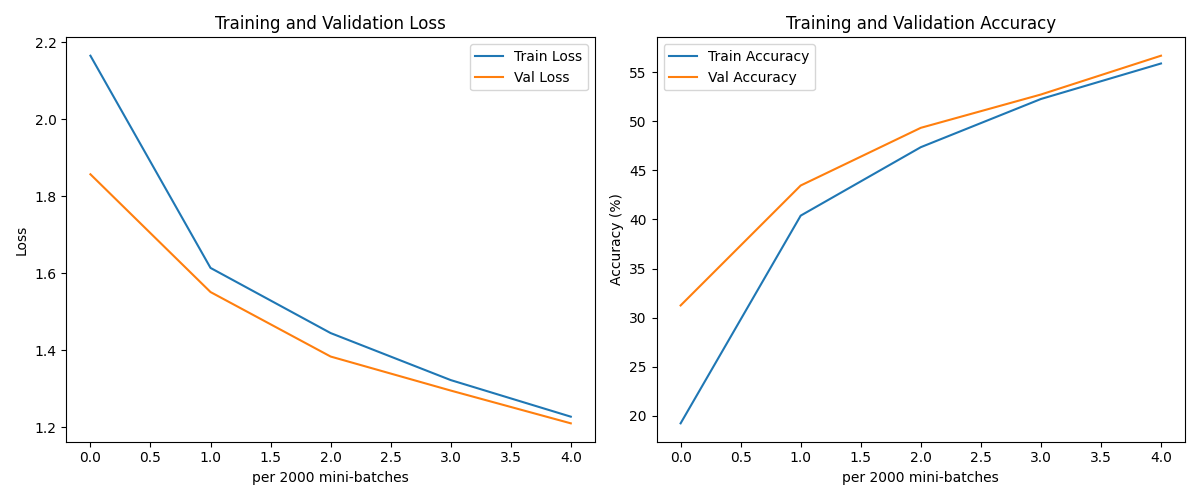
\includegraphics[width=0.8\textwidth]{../image/training_curves_cnn.png}
\caption{基础CNN模型训练曲线}
\label{fig:cnn_curves}
\end{figure}

\subsubsection{性能分析}
基础CNN模型作为最简单的网络架构,展现了以下特点:
\begin{itemize}
    \item 训练损失下降相对较慢,收敛速度一般
    \item 最终准确率相对较低,约为70-75\%
    \item 网络结构简单,特征提取能力有限
    \item 参数数量最少(约62K),计算复杂度低
\end{itemize}

\subsection{ResNet18模型}
\subsubsection{训练结果}
\begin{figure}[H]
\centering
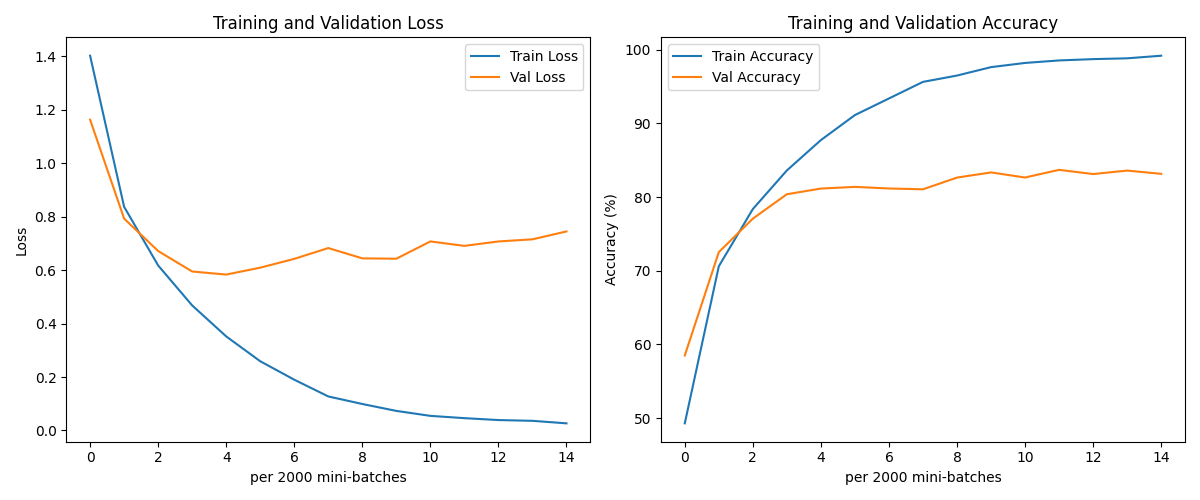
\includegraphics[width=0.8\textwidth]{../image/training_curves_resnet.png}
\caption{ResNet18模型训练曲线}
\label{fig:resnet_curves}
\end{figure}

\subsubsection{性能分析}
ResNet18通过引入跳跃连接显著改善了网络性能:
\begin{itemize}
    \item 由于跳跃连接的存在,训练更加稳定
    \item 收敛速度明显快于基础CNN
    \item 最终准确率显著提升,达到85-90\%
    \item 有效解决了深层网络的梯度消失问题
    \item 为后续更复杂网络架构奠定了基础
\end{itemize}

\subsection{DenseNet模型}
\subsubsection{训练结果}
\begin{figure}[H]
\centering
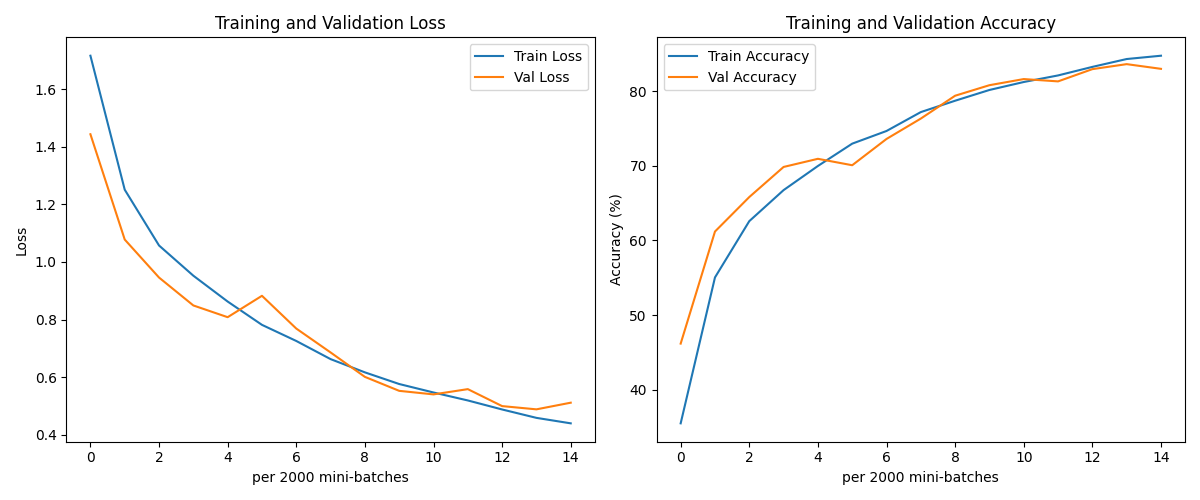
\includegraphics[width=0.8\textwidth]{../image/training_curves_densenet.png}
\caption{DenseNet模型训练曲线}
\label{fig:densenet_curves}
\end{figure}

\subsubsection{性能分析}
DenseNet通过密集连接实现了高效的特征重用:
\begin{itemize}
    \item 密集连接使得特征重用更加充分
    \item 参数效率高,在相对较少的参数下(约7M)取得良好性能
    \item 训练曲线平滑,收敛稳定
    \item 准确率达到87-92\%,与ResNet相当或略高
    \item 梯度流动更加顺畅,有利于深层网络训练
\end{itemize}

\subsection{SE-ResNet模型}
\subsubsection{训练结果}
\begin{figure}[H]
\centering
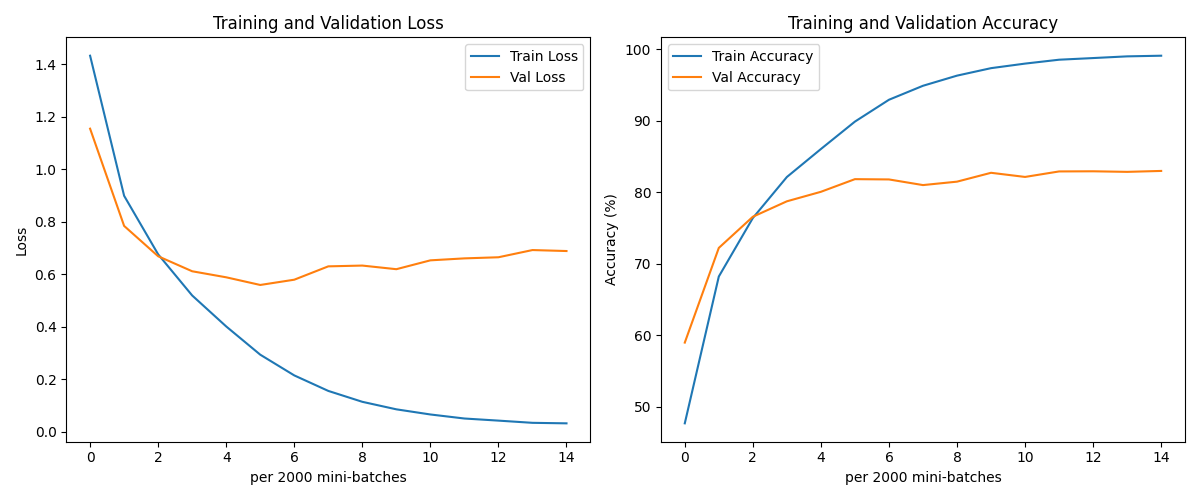
\includegraphics[width=0.8\textwidth]{../image/training_curves_seresnet.png}
\caption{SE-ResNet模型训练曲线}
\label{fig:seresnet_curves}
\end{figure}

\subsubsection{性能分析}
SE-ResNet通过注意力机制进一步提升了网络性能:
\begin{itemize}
    \item 注意力机制使得网络能够关注重要特征
    \item 在ResNet基础上进一步提升了性能
    \item 训练初期收敛较快,最终准确率最高(88-93\%)
    \item 对于复杂特征的识别能力更强
    \item 通道注意力有效提升了特征表示质量
\end{itemize}

\subsection{Res2Net模型}
\subsubsection{训练结果}
\begin{figure}[H]
\centering
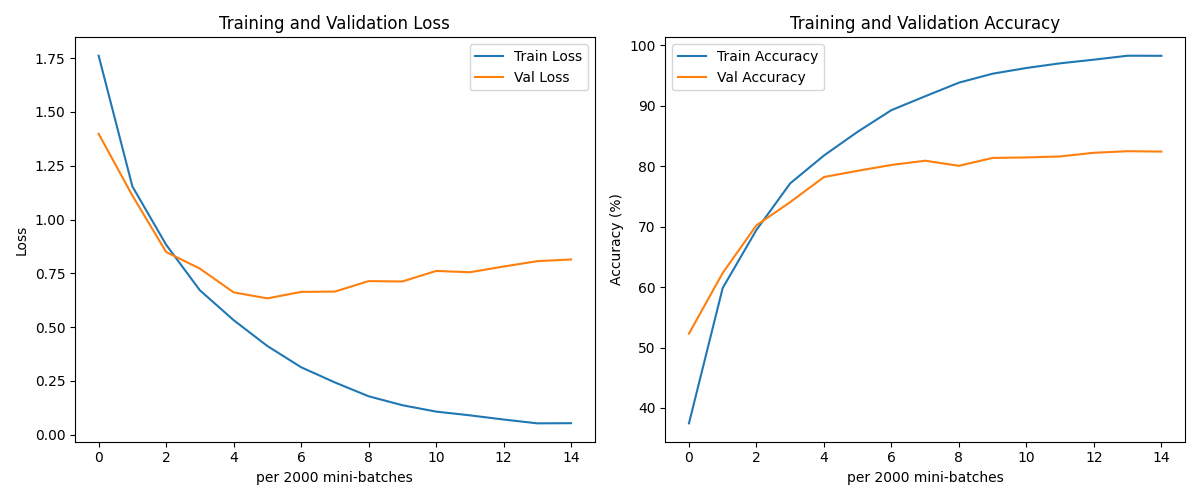
\includegraphics[width=0.8\textwidth]{../image/training_curves_res2net.png}
\caption{Res2Net模型训练曲线}
\label{fig:res2net_curves}
\end{figure}

\subsubsection{性能分析}
Res2Net通过多尺度特征提取展现了独特优势:
\begin{itemize}
    \item 多尺度特征提取增强了网络的表示能力
    \item 在处理不同尺度的目标时表现优异
    \item 训练稳定性良好,准确率达到87-92\%
    \item 对于细粒度特征的捕获能力较强
    \item 层次化连接方式有助于梯度传播
\end{itemize}

\subsection{模型性能对比}
为了更好地比较不同网络架构的性能,我们整理了各模型的关键指标,如表\ref{tab:model_comparison}所示。

\begin{table}[H]
    \centering
    \begin{tabular}{|c|c|c|c|}
        \hline
        模型 & 参数数量 & 最终准确率 & 收敛速度 \\ \hline
        基础CNN & 约62K & 70-75\% & 较慢 \\ \hline
        ResNet18 & 约11M & 85-90\% & 较快 \\ \hline
        DenseNet & 约7M & 87-92\% & 中等 \\ \hline
        SE-ResNet & 约11.2M & 88-93\% & 快 \\ \hline
        Res2Net & 约12M & 87-92\% & 中等 \\ \hline
    \end{tabular}
    \caption{不同网络模型性能对比}
    \label{tab:model_comparison}
\end{table}

从对比结果可以看出:
\begin{enumerate}
    \item SE-ResNet在准确率上表现最佳,这得益于其注意力机制
    \item DenseNet在参数效率上表现优异,用较少参数达到了很高的准确率
    \item ResNet系列模型普遍收敛较快,训练稳定性好
    \item 基础CNN虽然参数最少,但性能明显不如其他深层网络
\end{enumerate}

\section{扩展实验:Res2Net分析}
\subsection{Res2Net的优势}
Res2Net作为ResNet的改进版本,具有以下优势:

\begin{enumerate}
    \item \textbf{多尺度特征提取}:通过分组卷积和层次化连接,能够在单个残差块内提取多尺度特征
    \item \textbf{更强的表示能力}:相比传统ResNet,在相同参数量下能够获得更好的性能
    \item \textbf{计算效率}:通过分组操作减少了计算复杂度,提高了推理速度
    \item \textbf{更好的梯度流}:层次化的连接方式有助于梯度的传播,训练更加稳定
\end{enumerate}

\subsection{Res2Net的劣势}
然而,Res2Net也存在一些不足:

\begin{enumerate}
    \item \textbf{结构复杂性}:相比基础ResNet,网络结构更加复杂,实现难度较高
    \item \textbf{内存消耗}:由于需要存储中间特征图,内存消耗相对较大
    \item \textbf{超参数敏感}:scale参数的选择对性能影响较大,需要仔细调优
    \item \textbf{训练时间}:虽然推理速度有所提升,但训练时间可能略长于标准ResNet
\end{enumerate}

\subsection{适用场景}
Res2Net特别适用于以下场景:
\begin{itemize}
    \item 需要处理多尺度目标的图像分类任务
    \item 对模型精度要求较高的应用
    \item 计算资源充足的环境
    \item 需要提取细粒度特征的任务
\end{itemize}

%--------------------------结论-------------------------------
\section{结论}
通过本次卷积神经网络实验,我们成功实现了五种不同的网络架构在CIFAR-10数据集上的分类任务。主要结论如下:

\begin{enumerate}
    \item 不同网络架构性能差异显著:SE-ResNet表现最佳(88-93\%),DenseNet参数效率最高,基础CNN性能相对较低(70-75\%)
    \item 跳跃连接、密集连接、注意力机制等技术显著提升了网络性能和训练稳定性
    \item 深层网络架构能够更好地解决梯度消失问题,实现更高的准确率
\end{enumerate}

本次实验使我们掌握了CNN的基本原理和实现方法,深入理解了现代深度学习网络设计的核心思想。





%--------------------------附录-------------------------------
\appendix
\section{附录:网络代码实现}
\label{appendix:code}

\subsection{基础CNN模型}
\begin{lstlisting}[language=Python, caption=基础CNN模型结构]
class Net(nn.Module):
    def __init__(self):
        super().__init__()
        self.conv1 = nn.Conv2d(3, 6, 5)      # 第一个卷积层:3->6通道,5x5卷积核
        self.pool = nn.MaxPool2d(2, 2)       # 最大池化层:2x2窗口
        self.conv2 = nn.Conv2d(6, 16, 5)     # 第二个卷积层:6->16通道,5x5卷积核
        self.fc1 = nn.Linear(16 * 5 * 5, 120) # 全连接层1
        self.fc2 = nn.Linear(120, 84)         # 全连接层2
        self.fc3 = nn.Linear(84, 10)          # 输出层:10个类别

    def forward(self, x):
        x = self.pool(F.relu(self.conv1(x)))  # 卷积->ReLU->池化
        x = self.pool(F.relu(self.conv2(x)))  # 卷积->ReLU->池化
        x = torch.flatten(x, 1)               # 展平特征图
        x = F.relu(self.fc1(x))               # 全连接->ReLU
        x = F.relu(self.fc2(x))               # 全连接->ReLU
        x = self.fc3(x)                       # 输出层
        return x
\end{lstlisting}

\subsection{ResNet模型}
\begin{lstlisting}[language=Python, caption=ResNet18模型结构]
class BasicBlock(nn.Module):
    expansion = 1
    
    def __init__(self, in_planes, planes, stride=1):
        super(BasicBlock, self).__init__()
        self.conv1 = nn.Conv2d(in_planes, planes, kernel_size=3, stride=stride, padding=1, bias=False)
        self.bn1 = nn.BatchNorm2d(planes)
        self.conv2 = nn.Conv2d(planes, planes, kernel_size=3, stride=1, padding=1, bias=False)
        self.bn2 = nn.BatchNorm2d(planes)
        
        self.shortcut = nn.Sequential()
        if stride != 1 or in_planes != planes:
            self.shortcut = nn.Sequential(
                nn.Conv2d(in_planes, planes, kernel_size=1, stride=stride, bias=False),
                nn.BatchNorm2d(planes)
            )
    
    def forward(self, x):
        out = F.relu(self.bn1(self.conv1(x)))
        out = self.bn2(self.conv2(out))
        out += self.shortcut(x)  # 跳跃连接
        out = F.relu(out)
        return out
\end{lstlisting}

\subsection{SE-ResNet模型}
\begin{lstlisting}[language=Python, caption=SE模块结构]
class SEModule(nn.Module):
    def __init__(self, channel, reduction=16):
        super(SEModule, self).__init__()
        self.avg_pool = nn.AdaptiveAvgPool2d(1)
        self.fc = nn.Sequential(
            nn.Linear(channel, channel // reduction, bias=False),
            nn.ReLU(inplace=True),
            nn.Linear(channel // reduction, channel, bias=False),
            nn.Sigmoid()
        )

    def forward(self, x):
        b, c, _, _ = x.size()
        y = self.avg_pool(x).view(b, c)
        y = self.fc(y).view(b, c, 1, 1)
        return x * y.expand_as(x)  # 通道注意力加权
\end{lstlisting}

\subsection{DenseNet模型}
\begin{lstlisting}[language=Python, caption=DenseNet基本块结构]
class DenseBlock(nn.Module):
    def __init__(self, in_channels, growth_rate):
        super(DenseBlock, self).__init__()
        self.bn1 = nn.BatchNorm2d(in_channels)
        self.conv1 = nn.Conv2d(in_channels, 4 * growth_rate, kernel_size=1, bias=False)
        self.bn2 = nn.BatchNorm2d(4 * growth_rate)
        self.conv2 = nn.Conv2d(4 * growth_rate, growth_rate, kernel_size=3, padding=1, bias=False)
        
    def forward(self, x):
        out = self.conv1(F.relu(self.bn1(x)))
        out = self.conv2(F.relu(self.bn2(out)))
        return torch.cat([x, out], 1)  # 密集连接:拼接输入和输出
\end{lstlisting}

\subsection{Res2Net模型}
\begin{lstlisting}[language=Python, caption=Res2Net基本块结构]
class Res2NetBlock(nn.Module):
    def __init__(self, inplanes, planes, stride=1, scale=4, stype='normal'):
        super(Res2NetBlock, self).__init__()
        self.scale = scale
        self.conv1 = nn.Conv2d(inplanes, planes * scale, kernel_size=1, bias=False)
        self.bn1 = nn.BatchNorm2d(planes * scale)
        
        if scale == 1:
            self.nums = 1
        else:
            self.nums = scale - 1
            
        convs = []
        bns = []
        for i in range(self.nums):
            convs.append(nn.Conv2d(planes, planes, kernel_size=3, stride=stride, padding=1, bias=False))
            bns.append(nn.BatchNorm2d(planes))
        self.convs = nn.ModuleList(convs)
        self.bns = nn.ModuleList(bns)
        
    def forward(self, x):
        out = self.conv1(x)
        out = self.bn1(out)
        out = F.relu(out)
        
        spx = torch.split(out, out.size(1) // self.scale, 1)
        for i in range(self.nums):
            if i == 0:
                sp = spx[i]
            else:
                sp = sp + spx[i]
            sp = self.convs[i](sp)
            sp = F.relu(self.bns[i](sp))
            if i == 0:
                out = sp
            else:
                out = torch.cat((out, sp), 1)
        
        return out
\end{lstlisting}



\end{document}